\section{Design}

The previous section introduced all the methods we are going to be
using in this work in an abstract way. We will now go into the
practical implementation of everything: how we did it and why we did
it that way. We will describe the shortcomings or advantages of our
approaches and list tradeoffs we made to achieve our goals.

\subsection{Setup}

With our code living in a Git~\cite{Git} repository, we want to
achieve~-- aside from the obvious version control advantages~-- an
easily reproducible but also portable environment (by which we mean no
large binary files). We provide several individual scripts for the
whole setup pipeline of our environment, including the following:
\begin{itemize}
\item downloading the required tools (optionally also additional ones)
\item downloading the properly filtered hacks (as we established in
  section~\ref{sec:hacks}, these are in patch form)
\item decompressing them to properly named directories (supporting
  either \texttt{tar} or \texttt{7z} as desired)
\item applying the patches to the original ROM
\item dumping all levels in each ROM
\end{itemize}
All of these are combined in a single convenience script the user can
execute in order to obtain their own environment. We specify a default
directory structure our source code is based on so no paths have to be
changed if using the convenience script. Note that some patches, ROMs
and levels cause issues; we mentioned that these are listed in the
\texttt{stats} directory in section~\ref{sec:hacks}.

Some time after our download of the over 300~hacks, SMW Central
implemented protection against too many requests in a certain time
frame. Even though we have set a generous wait time limit between
downloads, we understand that troubling the servers over and over for
the same files may not be desired. Due to this, we supply scripts that
fetch the files (tools and hacks) from their original source, SMW
Central, and scripts that download the files collected in a custom
location provided by us (the convenience setup script exists in both
versions).

While we mentioned portability, the scripts above are currently only
implemented in shell script\footnote{Bash compatibility, aiming for
  POSIX.}. For cross-platform support, these will be implemented in
Julia as well at a later time, eliminating another dependency. \\
For people either not interested in a manual setup or without access
to a shell script interpreter, we provide downloads for pre-computed
databases in the dimensions we support out of the box (listed in
section~\ref{sec:preprocessing}). If, on the other hand, the levels
are available, generating those databases is done in a single function
call (\texttt{generate_default_databases()}).

Our repository contains pre-calculated values for several statistics
(these exist mostly to minimize the amount of layers we supply to the
models). However, when setting up manually, we recommend running the
functions \texttt{SMWLevelGenerator.Sprites.generateall()} and
\texttt{SMWLevelGenerator.SecondaryLevelStats.generateall()} to
pre-calculate statistics based on the user's dataset. If any of the
files containing statistics is not found, that statistic is otherwise
calculated on each load of the module. Depending on the size of the
dataset, this make take some time, therefore, pre-calculating will
speed up precompilation of the module.

Several other scripts allow further processing of the data, including:
\begin{itemize}
\item summarizing statistics of the hacks (like authors, rating,
  \dots)
\item removing duplicate levels based on their CRC32 checksums
\item removing levels with non-vanilla behavior
\end{itemize}
These have already been implemented in Julia.

%%% Local Variables:
%%% mode: latex
%%% TeX-master: "../../SMWLevelGenerator"
%%% End:


\subsection{Preprocessing}
\label{sec:preprocessing}

Our data was preprocessed so we obtain the following: A
space-efficient, performant, abstract level matching what we as humans
see. To actually get all those traits, we had to apply some tricks.
First, we need to establish the following: Remember that each level
may contain $30 \cdot 10^{6}$~entries at maximum~-- this requires
$30 \cdot 10^{6}\text{ bits} \div 8 = 3.75 \cdot 10^{6}\text{ bytes} =
3.75\text{ MB}$ (MB~are megabytes) of storage \emph{per level},
assuming we are able to compactly store eight entries per byte
(usually you need one byte per entry but as we have binary values, we
can store one value in one bit). With approximately 17\,000~levels, we
would then need
$3.75\text{ MB} \times 17\,000 \approx 63.75 \cdot 10^{3}\text{ MB} =
63.75\text{ GB}$ (GB~are gigabytes) of storage at maximum. While data
is cheap and this calculated number is the absolute maximum amount of
storage we may need, we would like our data to be more compact for
both efficiency and portability.

Even the data containing only layers of all tiles is so large that
keeping the full database in 8~gigabytes of memory is not
possible\footnote{This is the amount of unused RAM the author had
  available on his laptop while working with about 2\,000~browser tabs
  open.}. That means that creating a database is slower~-- as we would
have to partially write results to the file, garbage collect, then
restart with another partial result~-- and that reading, the much more
important part, is also slower as we would have to continually swap
out the database in memory (this is the effect on efficiency we
mentioned). As we want to train deep learning models which may require
many epochs over our data, this is not feasible since reading
gigabytes of serialized data is very slow.

To improve both space efficiency and performance during training, we
started using sparse arrays for larger data. Sparse arrays do not
store zeros; since our data is full of zeros (due to the binary
encoding which means we also have to store whether something is
\emph{not} at a position), we are able to save a lot of space and gain
a lot of speed due to improved computational techniques. We will not
have to iterate over our whole sparse array but only over the
non-zeros when computing a matrix-matrix-multiplication, for example.
Also, CUDA supports sparse arrays via the
\mbox{cuSPARSE}~\cite{CuSPARSE2012} library, enabling GPU-powered
sparse array computations as well (this sadly has not worked out yet,
as we explained in section~\ref{sec:julia}). Julia does not support
sparse arrays above two dimensions, so we needed to write our own
custom storage for 3-dimensional sparse arrays. While we managed to
greatly reduce storage space this way, it was still not enough for
storing all possible layers. Our two final optimizations were
compressing the indices of the sparse matrices to the smallest type
still being able to index and~-- because that was still not small
enough~-- only storing non-empty sparse matrices in an array. We wrote
a custom compressed sparse 3D~array format for that.

All in all, we now support four different compression levels with two
possible extensions based on compact bit arrays where each value fits
into one bit. The final size of the 3-dimensional database containing
all layers is roughly 430~MB if the highest compression level is used.
For sharing purposes, this data can be heavily compressed due to
recurring values, resulting in a 28~MB file when compressed with the
combination of \texttt{tar} and \texttt{gzip}. A
\mbox{7-Zip}-compressed file consumes about 16~MB of
storage\footnote{No special settings for \texttt{tar}, but the
  following command line options for \mbox{7-Zip}: \texttt{-t7z -mx9
    -m0=lzma2 -mmt2 -md1024m}}.
\medskip

While compression is great to share data, we are also interested in
speed. The usage of sparse arrays already nets us an increase in
calculations involving them. When not highly compressed, we store
3-dimensional data sliced along the second dimension, so by each layer
from left to right instead of from ``front to back''. To better
explain, remember that we \emph{do} store layers ``front to back'' for
the highest compression level; most layers of object types are empty
but most columns (slices from left to right) in the level are
not. \\
As a result, highly compressed data is stored in a way making it more
costly to bring it back together as caching suffers a lot when we need
each layer column by column (we would need to iterate over all layers
to get their first columns which we concatenate to obtain our first
input. This process has to be repeated for all columns).

Before we explain further, we should note the following: We create a
database for each ``type'' of training data, meaning models can
operate on well separated databases (which obviously comes at a cost
of space since data will be duplicated). It would also be possible to
work on one database containing all possible values at the cost of
speed due to having to convert all the data to the desired training
data\footnote{This has not been implemented.}. We separate the desired
training data by both its dimensionality and by the types of layers
contained in the data. These distinctions are relevant for database
generation, level generation and model creation as preprocessing
functions and the models need to know their input sizes ahead of time.

The dimensionality of training data is separated into three different
types to allow increasing model complexity:
\begin{enumerate}
\item 1-dimensional data containing only one row (or column for
  vertical levels) of one layer of the level. This row is computed in
  one of two ways (as given by the user): either the row is (1)~the
  row containing the maximum amount of values in the given layer or
  (2)~a combined row obtained by squashing all elements that are equal
  to 1 in the given layer vertically. See
  figure~\ref{fig:squash-example} for a simple visualization.

  To determine which layer to use by default (the tile we assume to be
  the ground tile for the level), we use a heuristic: we find the
  first non-empty tile below Mario's starting position\footnote{We
    mention this explicitly as the main entrance is two tiles above
    Mario's feet. Also, the empty tile is the tile corresponding to
    tile~37.}. If there is no non-empty tile below that position, we
  return the layer corresponding
  to tile~256, the default ground tile. \\
  It must be noted that this is not the correct tile for all levels.
\item 2-dimensional data containing only one layer of the level. The
  default layer is the same as for 1-dimensional data and suffers the
  same issues.
\item 3-dimensional data containing more than one layer of the
  level. By default, all layers are used.
\end{enumerate}

\begin{figure}[t]
  \centering
  \subfloat[Input]{%
    \centering
    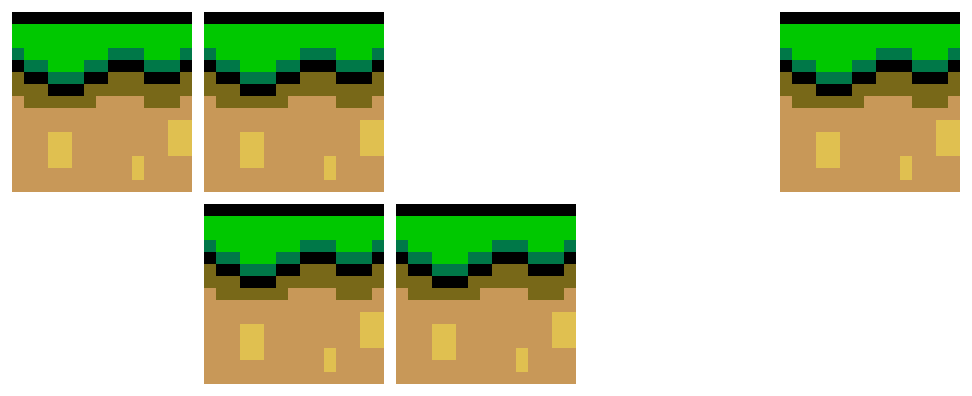
\includegraphics[width=0.5\textwidth]{squash_example.png}
  }\\
  \subfloat[\texttt{squash=false}]{%
    \centering
    
\includegraphics[width=0.5\textwidth]{squash_false.png}
  }\\
  \subfloat[\texttt{squash=true}]{%
    \centering
    
\includegraphics[width=0.5\textwidth]{squash_true.png}
  }%
  \caption{The two ways to obtain 1-dimensional data. Given (a)~as the
    input for either case, the outcome is either (b)~when taking the
    maximum over all rows or (c)~when squashing over all rows.}
  \label{fig:squash-example}
\end{figure}

Each of these can work on any combination of object types of data in
the level; for example, we can have 2-dimensional data containing only
Koopa sprites. Or 3-dimensional data containing only tiles and goal
sprites (as mentioned in the paragraph on layers on
page~\pageref{par:layers}, section~\ref{sec:levels}, we defined a
subset of the object type ``sprite'' containing only sprites directly
relevant to reaching the goal). With this, we can easily test models
on smaller data and adjust towards more complex problems.

For 3-dimensional data it is necessary to provide some information for
each of these combinations so that~-- as mentioned above~-- both data
loaders and models can properly handle different input sizes. \\
This information is the object types the data was created with and the
input size for sequence prediction models and GANs (the input sizes
will be calculated automatically in the future). Our system is easily
extensible to support any desired types; we only implemented the
following (as mentioned, only 3D~data needs extra implementations):
\begin{itemize}
\item \texttt{1d}: any 1-dimensional data
\item \texttt{2d}: any 2-dimensional data
\item \texttt{3dtiles}: 3-dimensional data containing all tile layers
\item \texttt{3d}: 3-dimensional data containing all layers
\end{itemize}
We also provide specific model creation functions for each of these
dimensionalities, giving the user simple access to the correct model
for each task. We will discuss this in detail in
sections~\ref{sec:generation-via-prediction}
and~\ref{sec:first-screen-generation}.

In this thesis, we work with data in column form. This means that our
models read levels column per column from the left to right. We
decided on this order as it captures elements in the past better than
reading the level row per row (where you go back and forth between the
start and end of the level). We also made it possible to read the
levels tile by tile if desired. The order is the same as for the
columns, reading from top to bottom, then from left to right. It is
also possible to change this order to read from bottom to top, then
from left to right. This may improve results at it may be more
important to first analyze the ground before predicting data above.

Now, we will summarize all the simplifications in our data set.

\subsubsection{Simplifications}
\label{sec:simplifications}

We already explained our simplifications in various locations above.
This is a comprehensive list of all of them:
\begin{itemize}
\item Levels are observed independently, meaning no connected levels
  are seen.
\item We omit a lot of metadata. (We suggest the omitted data is not
  related to level generation. As they are already parsed, including
  the omitted data is only a matter of uncommenting and adding a few
  lines of code, adjusting model inputs, and database generation.)
\item Test levels or unfinished levels~-- unless contained in the
  original game~-- are in the dataset.
\item Any data that is out of bounds is ignored (for example, sprites
  may ``fall down'' from a position above level bounds; we ignore
  those).
\item We assume that levels always go from left to right. This is only
  a problem during training as it arbitrarily makes training harder
  (only very few levels go from the right to the left). (We could
  determine whether the main entrance is at the left or right and
  horizontally flip the level accordingly. Even with this
  augmentation, handling levels with a starting position in the middle
  is simply not possible with our architecture.)
\item The type of tile that is assumed to be a level's ground
  (relevant for 1-~and 2-dimensional data generation) is determined
  heuristically (explained above; the first non-empty tile below
  Mario's starting position or tile~256 if none is found).
\item Levels that are (1)~vertical, (2)~boss levels or (3)~levels with
  layer~2 interaction are excluded.
\item Levels with modes deemed unusable by Lunar Magic are excluded.
\item Expanded levels (as designated by Lunar Magic) are excluded.
\item If the database contains a single sprite, we exclude all levels
  without a sprite header.
\end{itemize}

We will now explain our sequence prediction methods in detail.

%%% Local Variables:
%%% mode: latex
%%% TeX-master: "../../SMWLevelGenerator"
%%% End:


\subsection{Generation via Prediction}
\label{sec:generation-via-prediction}

We now focus on implementation details and design decisions regarding
our sequence prediction models. In the following explanations, we will
assume the level is read column per column. The only difference when
reading per tile is the input size. While each of our models may have
different input preferences for a sequence (vector of vectors, matrix,
\dots), we will focus our explanation on sequence elements as these
all follow the same principles. Each sequence element is a vector
consisting of
\begin{itemize}
\item a constant input part containing metadata,
\item a bit that indicates whether the level has not ended yet (so it
  is~1 if the level has not ended yet and~0 if this is the last column
  or beyond), and
\item a column (or single tile) of the level.
\end{itemize}
The constant input part supplies our model with the following
metadata:
\begin{itemize}
\item level number
\item amount of screens
\item level mode
\item level graphics (remember that these influence interactivity as well)
\item main and midway entrance action (these determine whether the
  level is a water level)
\item sprite buoyancy (how sprites interact with water)
\item disable layer~2 buoyancy (see above but for interaction with layer~2 data)
\item sprite mode
\end{itemize}
As mentioned, this list is easily extensible if desired as our
foundation contains and parses all relevant information.

To support many different models, we implement an abstract model class
(also called the ``model interface'') that requires extending only a
few methods for new models (if the provided defaults are not already
correct). One of these methods solves the problem of the desired input
for the model. Our data iterator will automatically shape the input
correctly for each model. The currently supported input types are
vectors of vectors and matrices. Single, long vectors containing the
whole sequence are implemented but some questions about how their data
is ordered must be answered individually (for example, is the constant
input provided only once or for each column like for the other input
types).

We implement a second loss function, the ``soft'' loss, that assigns a
lower penalty (or none) to sequence elements that were predicted
incorrectly if the prior two sequence elements were the same. With
this, we hope to de-regularize our models so they are less heavily
influenced by sudden changes in the level. The user may choose to use
either one during training (see section~\ref{sec:training-loops}).

By default, our LSTMs use the rectified linear unit activation
function~\cite{nairRectifiedLinearUnits,RectifierNeuralNetworks2019}
for hidden layers. Leaning on the original
implementation~\cite{OpenaiGpt22019}, we use the Gaussian error linear
unit activation function~\cite{hendrycksGaussianErrorLinear2018} for
the transformers. \\
It is important to note that our sequence prediction models do not
train on their own generated data which may improve results (this
could be done with a multitude of different steps into the future).
This is a large simplification heavily influencing any prediction
results on predicted data. As all the errors for each prediction will
accumulate, results will suffer accordingly.

The transformer models suffer from an issue in
\mbox{Transformers.jl}~\cite{peterChengchingwenTransformersJl2019} due
to the way batching works for these models (fixing this was out of the
scope of this work): We obtain a complete level matrix, a singular
input, by concatenating the preprocessed columns in the second
dimension; we then concatenate multiple of these matrices in the third
dimension to get a batch of inputs. As neither Julia nor cuSPARSE
provides support for sparse arrays in the third dimension, we are not
able to obtain perfect performance for the transformer models (as we
mentioned, cuSPARSE could not be used as of yet so this and the
following only affects data on the CPU at the moment). \\
This batching issue also has a large effect on memory usage as the
non-sparse data takes up a lot of space in high dimensions. For
3-dimensional data, a batch of 32~matrices of maximum length
(512~columns) would take
$58438 \cdot 32 \cdot 512 \cdot 2\text{ bytes} \approx 2 \cdot 10^{9} = 2\text{ GB}$ of data
(the first summand is the size of each sequence element) (we need
2~bytes per value due to the constant metadata inputs containing
16-bit values). Mapping this amount of data to a GPU that already
contains a large model is only possible in rare cases, so reducing
batch size, thereby decreasing efficiency, is the only option. In the
future, we will implement a wrapper around sparse matrices to act as a
3-dimensional array during computation for transformer models. \\
Even with these issues, our transformer models still mostly kept up
with or even outperformed the LSTM stacks, though this may be due to
inexperience on our side in choosing the correct amount of parameters.

We will now list the configuration options for our sequence prediction
models. As already mentioned, we provide convenience functions for
model creation for each training data dimensionality. As these are
only for convenience, they have some limitations\footnote{Obviously,
  any unlisted parameters can be changed manually by modifying the
  source code as well. This also goes for the models in the following
  sections.}.

LSTMs are built with the following parameters:
\begin{itemize}
\item amount of hidden layers
\item amount of hidden neurons per hidden layer
\item optional skip (or ``shortcut'')
  connections~\cite{heDeepResidualLearning2015} from each hidden layer
  directly to the final activation function
\item probability of dropout between every two hidden layers starting
  after the first one
\item final activation function
\end{itemize}
Our transformer creation functions take the following parameters:
\begin{itemize}
\item number of attention heads
\item hidden size of each attention head
\item hidden size of each fully connected layer
\item amount of transformer blocks
\item final activation function of each block
\item probability of dropout after attention layers and after each
  block
\item probability of dropout after fully connected layers
\item final activation function
\end{itemize}
The random model has a single parameter~-- its activation chance. By
default, it is set to the mean over the dataset for the appropriate
dimensionality (meaning the loss is optimal). \\
The input and output sizes are also adjustable for each model.

Having described the implementation details for our sequence
prediction models, we will now do the same for our GANs.

%%% Local Variables:
%%% mode: latex
%%% TeX-master: "../../SMWLevelGenerator"
%%% End:


\subsection{First Screen Generation}
\label{sec:first-screen-generation}

% TODO separate this conv part from dense wasserstein model
% TODO mention GPU clamping

In the following, we will describe implementation details of our GANs,
which each include a separate discriminator and generator model.
At first, we will only focus on DCGAN-based models.

First off, as mentioned in section~\ref{sec:julia}, we defined
convolutional layers without bias which were not included in Flux.jl
at the time of writing. \\
Our 1-dimensional GANs automatically adjust their layers to the input
size. The GANs for training data in 2D and above are implemented with
manually chosen stride, padding and dilation so the output is the same
size as the first screen of the level. The input to the discriminators
of our GANs is the first screen of the level (a vector of 16 elements
in the 1-dimensional case, a $27 \times 16$ matrix in the
2-dimensional case and a $27 \times 16 \times l$ cube in the
3-dimensional case, where $l$ is the amount of layers). Unlike our
sequence models, neither the discriminators nor the generators receive
any constant inputs of metadata (as the metadata is generated from the
GANs' outputs).

We use the same abstract model class for our GANs that was used for
the sequence prediction models, but extend it with two new classes for
discriminator and generator models. With this setup, we hope to make
extending the GAN pipeline with new models as simple as the sequence
prediction pipeline. Unlike the sequence predictors, discriminator
models do not allow inputs other than those of the form
$r \times c \times l \times b$ or $c \times l \times b$ (for the
1-dimensional case), where $r$ is the amount of rows, $c$ the amount
of columns, $l$ the amount of layers (channels in image processing)
and $b$ the batch size. We prodive layers to easily convert from this
format to a matrix and back (the matrix format is required for fully
connected layers). Generator models only take a vector of latent noise
of a size determined during model creation. This vector is only given
as a matrix due to batching (the model handles this automatically).

The first convolutional layer of the discriminator is not followed by
a normalization layer. We follow the example
of~\cite{PytorchExamples2019}
and~\cite{martinarjovskyMartinarjovskyWassersteinGAN2019}. The
discriminators use the leaky rectified linear unit activation function
for hidden layers while the generators use the standard rectified
linear unit activation.

We will now describe the differences of the fully connected GAN to the
DCGANs. The fully connected GANs automatically convert the inputs from
the batched form explained above to a matrix and back internally. They
also do not use batch normalization but instead have a dropout layer
every second layer starting from the first hidden layer onwards (just
like for the LSTMs but with fully connected layers instead of LSTM
layers; see section~\ref{sec:generation-via-prediction} for a more
detailed description).

Our DCGANs have the following parameters for their convenience
constructors (these are once again the same for the DCGAN and
Wasserstein DCGAN but with different defaults). It should also be
noted that while kernel size is adjustable, this requires building new
models as the expected sizes will be different. For the discriminators:
\begin{itemize}
\item amount of features in each convolutional layer's kernel; the
  features per successive layer are then multiplied by successive
  powers of two (starting from $2^{0}$ up to $2^{k - 2}$, where $k$ is
  the amount of convolutional layers\footnote{We get $k - 2$ because
    the start counting powers from zero and because the final
    convolutional layer shrinks the number of features to one.})
\item normalization layer after each convolutional layer
\item activation function after each normalization layer
\item final activation function
\item kernel window size
\end{itemize}
For the generators:
\begin{itemize}
\item amount of features in each convolutional layer's kernel; the
  features sizes follow the same rules as the discriminator but in
  reverse (starting form $2^{k - 2}$ and shrinking towards $2^{0}$,
  where $k$ is the amount of convolutional layers)
\item size of latent noise vector (the input size)
\item normalization layer after each convolutional layer
\item activation function after each normalization layer
\item final activation function
\item kernel window size
\end{itemize}
Finally, our fully connected GANs have the same parameters as the
LSTMs in section~\ref{sec:generation-via-prediction} except that the
final activation function can also be specified. Furthermore, the
generator accepts the size of the latent noise vector as well. \\
The input and output sizes are also adjustable for all model types.

After the GANs, the metadata predictor follows in our pipeline. That
model will be described in the next section.

%%% Local Variables:
%%% mode: latex
%%% TeX-master: "../../SMWLevelGenerator"
%%% End:


\subsection{Predicting Metadata}

This section lists implementation details for the final type of model
in this thesis: the metadata predictor. As mentioned in
section~\ref{sec:image-processing}, just like for GANs, there are
convolutional and fully connected models. These models receive the
same inputs as the discriminators described in
section~\ref{sec:first-screen-generation}. Similarly, the MLP-based
model correctly reshapes its inputs. \\
The convolutional metadata predictors were all manually created due to
the mix of convolutional and pooling layers. We use maximal pooling
layers, each followed by a dropout layer, throughout the network but
opt for average pooling as the last pooling operation before the fully
connected output layer.

Our models give as output the constant part of the inputs supplied to
the sequence predictors. Additionally, they output the bit which
indicates whether the level ends at this screen (also an input to the
sequence predictor; explained in
section~\ref{sec:generation-via-prediction}).

The convolutional metadata predictors have the following parameters:
\begin{itemize}
\item starting amount of features in each convolutional layer (these
  are multiplied by powers of two, first increasing, then decreasing.
  Due the models being hand-crafted, there is no clear formula; we
  therefore suggest a curious reader to take a look at the source
  code.)
\item probability of dropout
\item final activation function
\item kernel window size
\end{itemize}
The parameters of the MLP-based metadata prediction models are the
same as those for the MLP-based discriminators in
section~\ref{sec:first-screen-generation}.
As for all models, both the input and output size may be adjusted as well.

We have now not only described our methods in theory but also laid
them out practically, showing which options a casual user has and how
they affect the models internally. Next, we will combine the methods
to get our level generation pipeline.


%%% Local Variables:
%%% mode: latex
%%% TeX-master: "../../SMWLevelGenerator"
%%% End:


\subsection{Generating Levels}
\label{sec:generating-levels}

With the GAN outputs and the following metadata, the sequence
predictors have all the information they would get from a ``real''
level. Applying the models in sequence is one step; then we need to
reverse the whole preprocessing pipeline, converting our abstract
representation back to the correct formats that Lunar Magic can write
into the ROM. In this section, we will step through this pipeline one
by one. Once again, remember the high-level overview shown in
figure~\ref{fig:pipeline} on page~\pageref{fig:pipeline}.

We start with random input of the correct size for our generator,
apply it and get our first screen. At this point, we could also apply
our discriminator and retry generating the first screen if the emitted
value is too low. We have not implemented this feature. \\
The first screen is then fed into the metadata predictor, giving us
the generated level's metadata. This constant input is then combined
with the level in the correct specification, depending on whether the
sequence predictor accepts columns or singular tiles, and all but the
last sequence elements have their ``sequence has not ended yet''-bit
set to~1. \\
The data is now in the same format as a preprocessed real level and we
apply the sequence prediction model sequentially until we either find
that the ``sequence has not ended yet''-bit is~0 or until the maximum
level length is reached. This complete output is then postprocessed.

As we skipped some metadata when preparing our data, we need to fill
the omissions with default values. For all unknown data, we chose
either the defaults of level~261, the first level Lunar Magic presents
to the user, or give ``empty'' values if possible. Before we give an
example, remember that Lunar Magic dumps sprite data in a ``.sp'' file
containing the sprite header and then data of individual sprites in
the level until a designator for the ending is encountered. If our
model does not generate sprites, we don't write back the sprites in
level~261 but instead set the sprite header to that of level~261 but
do not give any sprites themselves. While the sprite header is
required, sprites are not.

Generation functions include generating a single level or multiple
levels. A function to generate a whole hack of levels (meaning
512~different levels, each with a different number) is planned. We
also implement model-specific generation functions. For the sequence
prediction model, functions may generate levels like the above
functions or based on predicting on the original game's levels. The
GANs may also generate only the first screen for a level
independently.

Note that during all of this, the user does not have to worry about
dimensionality in any way; all of this is handled automatically if the
model was supplied the correct parameters (such as its
dimensionality). We allow writing back 1-dimensional outputs by
hardcoding the default row the generated output should be placed in
and by filling the rest of the level with empty tiles.

We will now dive into implementation details and design decisions
regarding our training pipeline, the most important part of our
program that first enables our models to generate meaningful outputs.

%%% Local Variables:
%%% mode: latex
%%% TeX-master: "../../SMWLevelGenerator"
%%% End:


\subsection{Training Pipeline}
\label{sec:training-pipeline}

Our training pipeline for each type of model consists of two major
parts: the data iterator which reads and preprocesses our data and the
actual training loop acting on the data we obtain from the iterator. \\
Let us first focus on the data iterators and after that on the
training loops.

\subsubsection{Data Iterators}

Since the data iterator is responsible for shaping our data to the
form expected by the model, we still need to apply some more
preprocessing to the already preprocessed data contained in the
database. As this may be a large bottleneck, we focused on optimizing
data iteration (on any 1.3-version and above of Julia, this bottleneck
can mostly be avoided by simply using enough data iterator threads).
As we explained in section~\ref{sec:preprocessing}, our data is stored
differently if using the highest compression level. We also explained
that storing our 3-dimensional data in ``columnar'' layers (sliced
along the second dimension) is more performant. With the columnar
format, we can simply concatenate the individual matrices and obtain
our level in a cache-efficient way. \\
All data iterators use thread-safe channels which the user can take
values out of without having to worry about race conditions and
synchronicity.

We do not normalize our data in any way. Normalizing the mean would
mean losing the sparsity patterns which improve computational
efficiency by a large margin. We decided against normalizing the
covariance due to the differences in the way we shape our data for
each model and the subsequent influences on unrelated results. First
off, we cannot calculate the covariance of the unmodified dataset due
to the differences in sequence lengths. While we could easily compute
the covariance of our dataset by padding all sequences to the same
length, using this result to normalize data for \emph{all} models
would affect~-- for example~-- sequence models that allow sequences of
different lengths in an undesired way. This is because we normalize
their input data based on data that is nonexistent in their view (the
padded zeros).

With the added randomness of the order the data iterator threads
output their data (due to operating system scheduling and other
factors~-- this randomness is not affected by a random number generator
seed), we cannot guarantee reproducible results if using threads.
While we could adjust the iterators to synchronize so results are
perfectly reproducible, we decided to not implement this feature as we
assume this would largely hinder efficiency. In the future, an option
to enable perfect reproducibility would be a good improvement. \\
To minimize overhead, we keep each thread running in an endless loop,
meaning the user needs to keep track of how many training examples
they need for each epoch. In an earlier implementation, an iterable
data iterator was used but we decided this minor convenience was not
worth having to start multiple threads on each training and test
epoch.

The data iterator for first screen data works similar to the other but
has fewer options as we do not need to iterate over the first screen
but supply it as a whole. With this, we do not need to handle possibly
iterating over each tile and~-- with that option activated~-- in which
direction to iterate (each ``columnar'' slice from top to bottom or
bottom to top). We also have not found the need to worry about padding
and supporting different inputs for different models (as of yet).
Obviously, we still need to support the different dimensionalities of
data. \\
This data iterator also supplies a tuple of values for simplicity: the
first screen and the constant input of each level. This enables us to
reuse the iterator for both GAN and metadata predictor training.

\subsubsection{Training Loops}
\label{sec:training-loops}

Our training loops for all model types follow the same schematic:
\begin{enumerate}
\item Initialize parameters, data iterators, loggers, optionally load
  model, \dots
\item Store parameters
\item Initial test
\item Loop over all epochs:
  \begin{enumerate}
    \item Train model(s)
    \item Periodically test model and check for early stopping
    \item Periodically save model checkpoint
  \end{enumerate}
\item Save model checkpoint
\item Clean up resources
\end{enumerate}

All training loops accept either a model or the path to a model
checkpoint, correctly initializing everything from the checkpoint and
starting training from the exact point it left off (although this may
not always be the exact point due to the randomness in threaded data
iterators; we skip as many steps as are saved in the checkpoint). The
parameters that are the same over all training loops contain values
like the number of epochs, early stopping-related values, which
checkpointing method to use (as discussed in section~\ref{sec:julia},
we support saving as BSON or JLD2), after how many training steps to
log and save the model, the amount of data iterator threads, the
random seed and others. \\
The parameters are collectively combined with parameters stored in the
model (an optional specification of our abstract model interface) and
saved in a JSON file to combine both human readability and parsing.

We already mentioned in section~\ref{sec:generation-via-prediction}
that our sequence prediction models implement a ``soft'' loss
function; these are also selected as a training parameter. \\
Due to the iterator allowing it, the GAN training loop allows training
both a GAN and a metadata predictor at the same time.

%%% Local Variables:
%%% mode: latex
%%% TeX-master: "../../SMWLevelGenerator"
%%% End:



%%% Local Variables:
%%% mode: latex
%%% TeX-master: "../SMWLevelGenerator"
%%% End:

